\documentclass[../../report.tex]{subfiles}
\begin{document}
\section{Previous Work}

During the initial stages of research for this project, I was not able to find
any substantial previous attempts at symbolic melody generation with SNNs.
Therefore, the implementation was largely guided by SNN experiments in other
tasks \cite{Bellec2020, Bellec2018LSNN}. It was also useful to analyse ANN-based
approaches to this task, and one of the biggest sources of inspiration was
Google's \emph{Magenta}, an open source research project exploring the role of
machine learning in creativity.

\subsection{Melody RNN}

Soon after its inception, Magenta began work on monophonic MIDI generation
models, all based on a two-layer LSTM with \emph{one-hot}\footnotemark{} melody
encoding. The first model in this series is Basic RNN \cite{Abolafia2016}. Here,
the input and output is limited to a span of 3 octaves (C3 -- C6). Melodies
generated by this model exhibit convincing local contours, but at a larger
scale, the melody wanders, failing to stick to a single theme. Nevertheless, the
simplicity of Basic RNN leaves a lot of room for modification, and thus its code
was used as a foundation for the SNN model.

\footnotetext{One-hot encoding is a method of representing categorical data,
e.g. musical notes. It transforms a single data point into an array whose size
is equal to the number of distinct categories. This array contains a `1' in the
position of the relevant category, and `0' elsewhere.}

Lookback RNN \cite{Waite2016} builds on top of the basic configuration by
augmenting the melody encoding. It includes additional event categories that
allow the model to `look back' in time and repeat notes generated 1 or 2 bars
ago. This aims to capture the repetition patterns common in popular Western
music. From my own experiments with this model, I found that these `training
wheels' indeed allow the model to hold on to musical motifs in short melodies,
however its memory still fades in longer sequences.

Attention RNN \cite{Waite2016} further improves melody cohesion. With the help
of an \emph{attention} mechanism, the model can access several previous RNN
states in each computation step. This means that it is not required to encode
all of the relevant information in a single vector, which allows the model to
make better decisions by considering its previous `state of mind'.

\subsection{Performance RNN}

The qualities of music that make it enjoyable are much more subtle than the mere
ordering of notes. Melody RNN largely ignores the notion of \emph{expression} by
quantising constant-velocity\footnotemark{} notes to a fixed time step.
Performance RNN \cite{Simon2017} addresses this issue by handing over time and
velocity controls to the model, rather than the output decoding pipeline. This
results in melodies that sound much more natural, albeit still lacking long-term
structure.

\footnotetext{In the context of MIDI, velocity refers to the triggering force of
a note, which usually affects the loudness of the produced sound.}

\subsection{Music Transformer}

The latest and best symbolic music generation model to come from Magenta is
Music Transformer \cite{Huang2018}. It is based on and named after the
Transformer \cite{Vaswani2017}, an attention based network architecture for
sequence processing. More importantly, the Transformer abandons sequential
computation, which is a major performance bottleneck in RNNs. Among all the
models described in this section, this one is superior in terms of long-term
cohesion (figure \ref{fig:transformer-attention}).

\begin{figure}
  \centering
  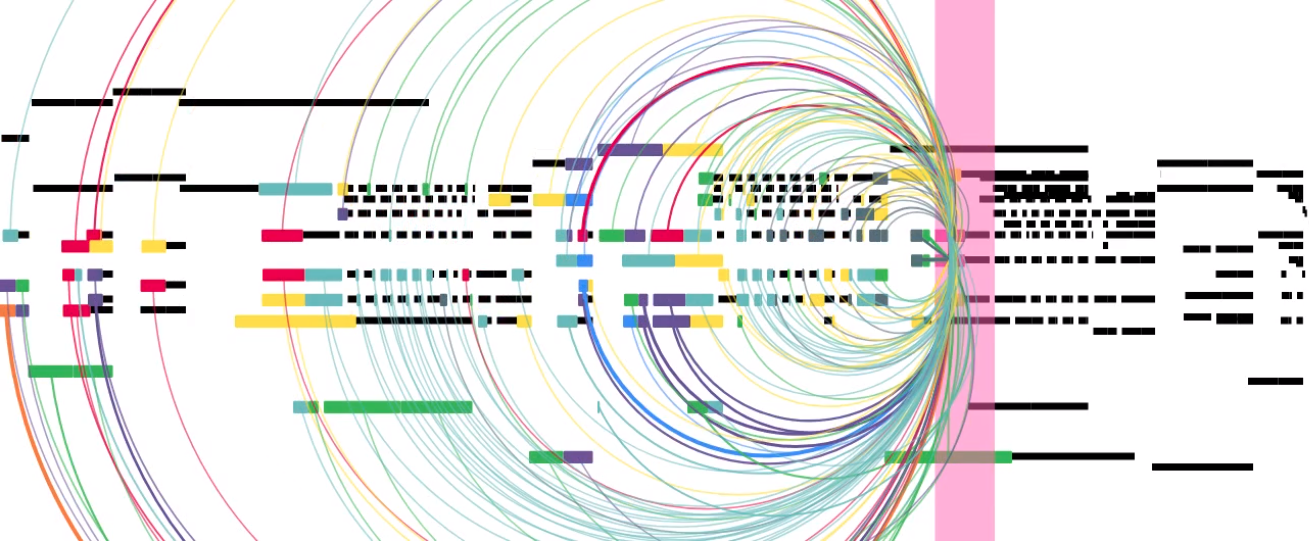
\includegraphics[width=\textwidth]{transformer-attention}
  \caption{To generate the next note (pink stripe), Music Transformer's many
  \emph{attention heads} (each in a different colour) consider preceding notes
  at multiple timescales. Attention weight is represented by arc thickness.
  \cite{Huang2018Visual}}
  \label{fig:transformer-attention}
\end{figure}

\end{document}
